%Starting.
\pgfdeclarelayer{frontmost}
\pgfdeclarelayer{colnameslayer}
\pgfsetlayers{main,frontmost,colnameslayer}
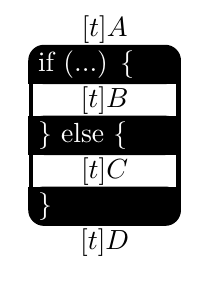
\begin{tikzpicture}[x=1mm,y=1mm,scale=1.]
% State has been set.
\begin{pgfonlayer}{frontmost}
\draw [black] (11.,-3.) node{\smash{$\ml[t]{A}$}};
\end{pgfonlayer}
\draw [line width = 0.6mm, black] (1.65,-10.) -- (1.65,-9.);
\draw [line width = 0.6mm, black] (20.35,-10.) -- (20.35,-9.);
\fill[fill=black, rounded corners=2.mm] (1.3,-9.) rectangle (20.7,-4.);
\fill[fill=black] (1.3,-9.) rectangle (20.7,-6.5);
\draw [white] (1.3,-6.5) node[anchor=west]{\code{if (...) \{}};
\draw [line width = 0.6mm, black] (1.65,-13.) -- (1.65,-9.);
\draw [line width = 0.6mm, black] (20.35,-13.) -- (20.35,-9.);
\begin{pgfonlayer}{frontmost}
\draw [black] (11.,-12.) node{\smash{$\ml[t]{B}$}};
\end{pgfonlayer}
\fill[fill=black, rounded corners=2.mm] (1.3,-18.) rectangle (20.7,-13.);
\fill[fill=black] (1.3,-15.5) rectangle (20.7,-13.);
\fill[fill=black] (1.3,-18.) rectangle (20.7,-15.5);
\draw [white] (1.3,-15.5) node[anchor=west]{\code{\} else \{}};
\draw [line width = 0.6mm, black] (1.65,-18.) -- (1.65,-13.);
\draw [line width = 0.6mm, black] (20.35,-18.) -- (20.35,-13.);
\draw [line width = 0.6mm, black] (1.65,-22.) -- (1.65,-18.);
\draw [line width = 0.6mm, black] (20.35,-22.) -- (20.35,-18.);
\begin{pgfonlayer}{frontmost}
\draw [black] (11.,-21.) node{\smash{$\ml[t]{C}$}};
\end{pgfonlayer}
\draw [line width = 0.6mm, black] (1.65,-22.) -- (1.65,-21.);
\draw [line width = 0.6mm, black] (20.35,-22.) -- (20.35,-21.);
\fill[fill=black, rounded corners=2.mm] (1.3,-27.) rectangle (20.7,-22.);
\fill[fill=black] (1.3,-24.5) rectangle (20.7,-22.);
\draw [white] (1.3,-24.5) node[anchor=west]{\code{\}}};
\begin{pgfonlayer}{frontmost}
\draw [black] (11.,-30.) node{\smash{$\ml[t]{D}$}};
\end{pgfonlayer}
\end{tikzpicture}
%Finished.
